%%%%%%%%%%%%%%%%%%%%%%%%%%%%%%%%%%%%%%%%%%%%%%%%%%%%%%%%%%%%
% ATTENTION !!!!!
% Ne pas écrire ici, ce fichier est fait pour la mise en page
% Pour écrire, éditer le fichier portant le nom de la partie 
%%%%%%%%%%%%%%%%%%%%%%%%%%%%%%%%%%%%%%%%%%%%%%%%%%%%%%%%%%%%

%%%% Packages utilisés pour ce rapport
\documentclass[12pt,openany]{report} %taille de police et type de document
\usepackage[utf8]{inputenc} % type d'encodage
\usepackage[francais]{babel} % pour le respect des règles typographique française
\usepackage{lmodern} % paquet de police (ressemble à time new roman) 

\usepackage{fullpage} % pour gérer les tailles de marges
\usepackage{fancyhdr} % pour plus d'option de mise en page
\usepackage{titlesec} % permet de gérer la mise en page des titres
\usepackage{hyperref} % pour avoir des lien hypertexte
\usepackage{setspace} % pour l'espace interligne

\usepackage{gensymb} % 3 paquets pour les expression mathématiques
\usepackage{amsmath}
\usepackage{amssymb}

\usepackage{tocloft} % pour les tables de matières, de figures et de tableaux
\usepackage{graphicx} % pour inclure des images
\usepackage{caption} % pour les légendes
\usepackage{listingsutf8} % pour l'ajout de code

\usepackage{multicol} % pour écrire du texte dans plusieurs colonnes
\usepackage{minitoc} % pour plus d'option de mise en page

\usepackage[toc,page]{appendix}
\usepackage{cleveref}


\pagestyle{fancy}
\lhead{}
\chead{}
\rhead{}
\lfoot{}
\cfoot{}
\rfoot{\thepage}
\renewcommand{\headrulewidth}{0pt}
\renewcommand{\footrulewidth}{0pt}

\fancypagestyle{plain}{
	\lhead{}
	\chead{}
	\rhead{}
	\lfoot{}
	\cfoot{}
	\rfoot{\thepage}
	\renewcommand{\headrulewidth}{0pt}
	\renewcommand{\footrulewidth}{0pt}
}

\onehalfspacing

%titre, auteur, date
\title{Introduction à l'utilisation d'un système GNU/LINUX}
\author{Nicolas Cubric\\Association Robotronik Phelma}
%\date{}

% début du document
\begin{document}
%Formattage des titres de chapitre, section, sous-section
\titleformat{\chapter}[block]{\bf\huge}{\thechapter}{2pc}{}   
\titlespacing*{\chapter}{0pt}{-30pt}{15pt}
\renewcommand\thechapter{\Roman{chapter}}

\titleformat{\section}[block]{\bf\Large}{\thesection}{2pc}{}
\renewcommand\thesection{\thechapter.\arabic{section}}

\titleformat{\subsection}[block]{\bf\large}{\thesubsection}{2pc}{}
\renewcommand\thesubsection{\thesection.\arabic{subsection}}


%Formattage du titre du sommaire
\setlength{\cftbeforetoctitleskip}{-2em}

\makeatletter

% page de garde
\begin{titlepage}
	\begin{center}
		\begin{minipage}{\linewidth}
			\begin{minipage}{0.5\linewidth}
				
\includegraphics[width=0.5\linewidth]{Images/logo_phelma.jpg}
			\end{minipage}
			\hspace{0.25\linewidth}
			\begin{minipage}{0.5\linewidth}
				
\includegraphics[width=0.5\linewidth]{Images/logoclub.jpg}
			\end{minipage}
		\end{minipage}


		\vfill

		{\large \textbf{}}\\
		\vspace*{1cm}
		{\LARGE\textbf{\@title}}

		\vfill

		
\includegraphics[width=0.5\textwidth]{Images/tux.png}

		\vfill

		{\large\emph{} \textbf{}}\\
		\vspace*{0.5cm}
		{\large\textbf{\@author}}\\

		\vfill

		{\large \@date}
	\end{center}
\end{titlepage}

\include{Remerciements}

%Sommaire, tables des figures et des tableaux
\renewcommand{\contentsname}{Sommaire}
\tableofcontents
\clearpage

\listoffigures
\clearpage

\listoftables
\clearpage

\chapter{Linux c'est quoi ?}

Linux ou plus précisément GNU/Linux est un système d'exploitation basé sur un noyau UNIX. À la différence de Windows, qui est basé sur un noyau DOS, Linux est open source, c'est à dire que tout le monde peut avoir accès aux code sources et les modifiés à sa guise. La seule règle étant de laisser son œuvre libre et disponible à tous.


\chapter{L'arborescence}

L'arborescence sous Linux correspond à la manière sont agencés les dossiers (directory en anglais) les uns par rapport aux autres.

\begin{center}
	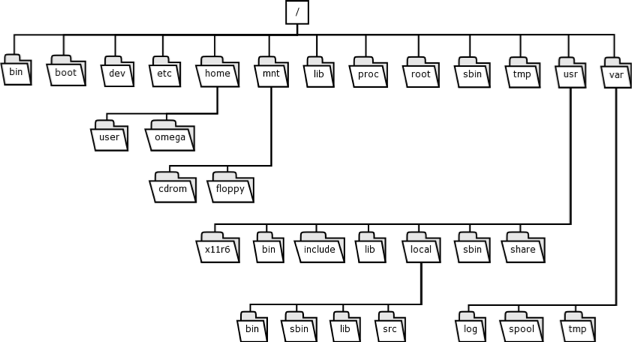
\includegraphics[width=0.7\textwidth]{Images/arborescence.png}
	\captionof{figure}{Arborescence d'un système GNU/Linux}
\end{center}

Vous l'aurez peut être remarqué mais tous les dossiers mènent à /. Ce dossier a pour petit nom, root. Il est ce que l'on appelle la racine du système. De ce dossier découle une floppé d'autre. Chacun à son utilité, nous allons voir les "plus important"
\begin{itemize}
	\item home : ce dossier contient les fichiers des utilisateurs. C'est ici que se situe les données des utilisateurs.
	\item 
\end{itemize}

\chapter{Commandes de bases}

Dans cette partie, nous allons voir les commandes de bases qui permettent de se débroullier dans un terminal.


À la différence de Windows, le terminal est un outils très utilisé sous linux. Il permet de :
\begin{itemize}
	\item se déplacer dans l'arborescence des fichiers
	\item créer/supprimer des dossiers
	\item créer/éditer/supprimer des fichiers
\end{itemize}

Évidemment il existe des outils graphiques pour effectuer ces différentes tâches mais parfois il peut être plus rapide de faire ces actions diretement dans le terminal.

\section{pwd (print working directory)}
Cette commande permet de savoir où l'on se situe dans l'arborescence.

\begin{center}
	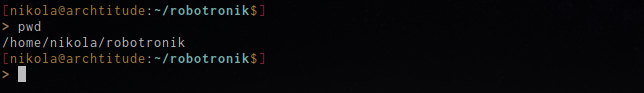
\includegraphics[width=0.6\textwidth]{Images/pwd.png}
	\captionof{figure}{Sortie de la commande pwd}
\end{center}

\section{ls}
Cette commande permet de lister les éléments présents dans un dossier.

\begin{center}
	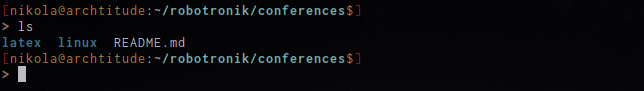
\includegraphics[width=0.6\textwidth]{Images/ls.png}
	\captionof{figure}{Sortie de la commande ls}
\end{center}

Il est possible d'ajouter des flags (drapeaux) à cette commande. Les flags sont des options que l'on peut affecter à une commande. La plupart du temps, la liste des flags affectable à une commande peuvent être trouver dans le manuel de cette commande.

Par exemple, si l'on ajoute le flag -a :

\begin{center}
	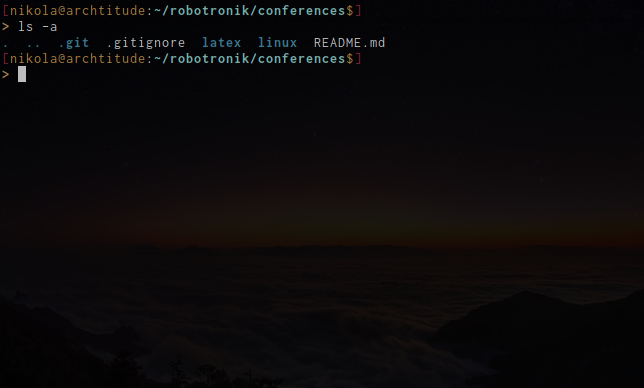
\includegraphics[width=0.6\textwidth]{Images/ls-a.png}
	\captionof{figure}{Sortie de la commande ls -a}
\end{center}

De nouveaux fichiers sont apparus. Le nom de ces fichiers est précédé d'un point. Cela signifie que ce sont des fichiers cachés. Si l'on demande pas de les afficher explicitement il ne seront pas visibles.

Plusieurs flags peuvent être utilisés en même temps. Par exemple, si l'on entre la commande :
\begin{lstlisting}[language=bash]
	ls -al
\end{lstlisting}

\begin{center}
	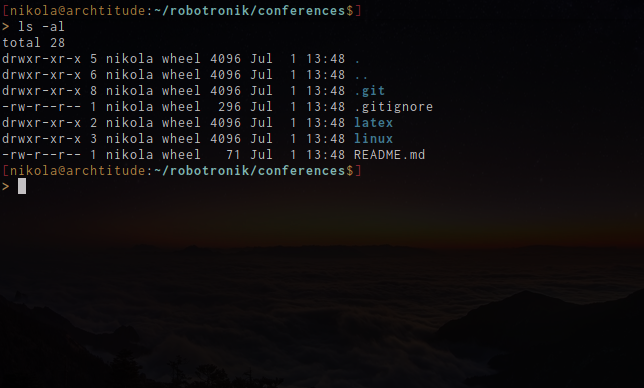
\includegraphics[width=0.6\textwidth]{Images/ls-al.png}
	\captionof{figure}{Sortie de la commande ls -al}
\end{center}

Ici, les fichiers cachés sont toujours affiché car nous avons mis le flag a mais l'affichage est changé. Cela est dû au flag -l qui permet d'obtenir plus d'inofrmation sur les fichiers commes leur taille, leurs autirisations, leur propriétaire et leur date de dernière modification.

\section{cd (change directory)}
Cette commande permet - comme son nom l'indique - de changer de dossier.

\begin{center}
	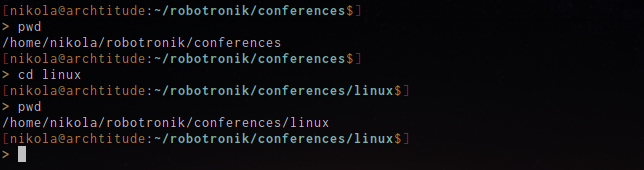
\includegraphics[width=0.6\textwidth]{Images/cd.png}
	\captionof{figure}{Sortie de la commande cd}
\end{center}

\section{mkdir (make directory) / rmdir (remove directory)}
Ces deux commandes permettent de créer et supprimer des dossiers.

\begin{center}
	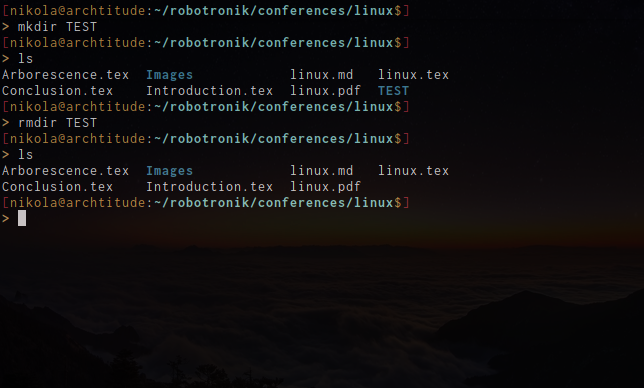
\includegraphics[width=0.6\textwidth]{Images/dir.png}
	\captionof{figure}{Création puis suppression d'un dossier}
\end{center}

Attention pour utiliser rmdir, il faut que le dossier que l'on veut supprimer soit vide. Sinon il faut utiliser la commande rm (cf \ref{sec:touch-rm})

\section{touch/rm}\label{sec:touch-rm}
Ces deux commandes permettent de créer et supprimer des fichiers. 

La commande touch ne permet de créer que des fichiers et non des dossiers. Pour créer un fichier il faut entrer cette commande :
\begin{lstlisting}[language=bash]
	touch nom_de_mon_fichier.extention_de_mon_fichier
\end{lstlisting}

Par exemple, disons que l'on veut créer un fichier pour ecrire un programme en C :

\begin{center}
	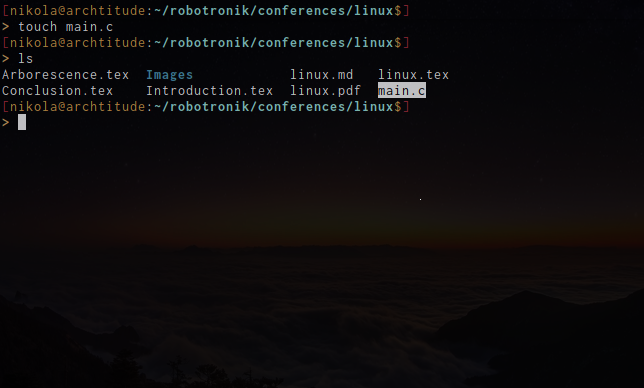
\includegraphics[width=0.6\textwidth]{Images/touch.png}
	\captionof{figure}{Création du fichier main.c}
\end{center}

La commande rm permet de supprimer un élément. Elle pernet aussi de supprimer des dossiers non vide en lui affectant les bons flags.

\begin{center}
	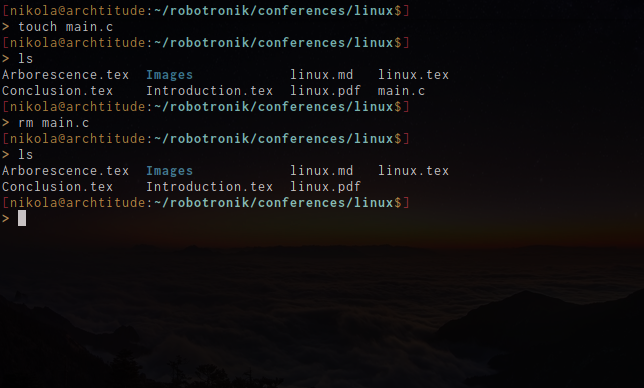
\includegraphics[width=0.6\textwidth]{Images/rm.png}
	\captionof{figure}{Suppression du fichier crée précédement}
\end{center}



% bibliographie
% \addcontentsline{toc}{chapter}{Bibliographie}
% \bibliographystyle{apalike}
% \bibliography{biblio.bib}
% % pour inserer des références pas citées dans le texte
\nocite{}

\end{document}

